\documentclass[../main.tex]{subfiles}

\graphicspath{{../images/}}

\begin{document}
\pagestyle{fancy}
\lhead{Homework 6}
\chead{Junseo Shin}
\rhead{PHYS 421}

\setcounter{section}{6}
% 4.1, 4.2, 4.8, 4.11, 4.14, 4.34

\paragraph{4.1} 
Given the Polarizability of Hydrogen atom
\begin{align*}
    \frac{\alpha}{4\pi\epsilon_0} = \qty{0.667e-30}{m^3}
\end{align*}
of bohr radius $a = \qty{0.5e-10}{m}$,
and the E-field between metal plates separated $\Delta D = \qty{1e-3}{m}$ apart and connected to a 500 V battery is
\begin{align*}
    E = \frac{V}{\Delta D} = \frac{\qty{500}{V}}{\qty{1e-3}{m}} = \qty{5e5}{V/m}
\end{align*}
The dipole moment is ($\epsilon_0 = \qty{8.85e-12}{\frac{C^2}{N.m^2}}$)
\begin{align*}
    p = \alpha E = qd \implies d = \frac{\alpha E}{q} = \frac{(4\pi \epsilon_0) \qty{0.667e-30}{m^3} \times \qty{5e5}{V/m}}{\qty{1.6e-19}{C}} = \qty{2.32e-16}{m}
\end{align*}
So the separation distance $d$ as a fraction of the atomic radius $a$ is
\begin{align*}
    \boxed{
        \frac{d}{a} = \frac{\qty{2.32e-16}{m}}{\qty{0.5e-10}{m}} = \num{4.6e-6}
    }
\end{align*}
The estimate voltage we need to ionize the atom is 
\begin{align*}
    V &= E \Delta D, \quad E = \frac{qd}{\alpha} \\
    \implies V  &= \frac{qa}{\alpha} \Delta D = \frac{\qty{1.6e-19}{C} \times \qty{0.5e-10}{m}}{(4\pi \epsilon_0)\qty{0.667e-30}{m^3}} \times \qty{1e-3}{m} = \boxed{\qty{1.1e8}{V}}
\end{align*}

\newpage
\paragraph{4.2}
Given the charge density of a groundstate hydrogen atom
\begin{align*}
    \rho (r) = \frac{q}{\pi a^3} e^{-2r/a}
\end{align*}
where $q$ is the electron charge and $a$ is the Bohr radius, find the atomic polarizability. 

FIrst calculating the electric field of the electron cloud
\begin{align*}
    E_e (r) &= \ke \frac{Q}{r^2}
\end{align*}
where the enclosed charge $Q$ is
\begin{align*}
    Q &= \int \rho(r') \dd \tau, \quad \dd\tau = r^2 \sin\theta \dd r \dd\theta \dd\phi \\
    &= \frac{q}{\pi a^3} (4\pi) \int_0^r r'^2 e^{-2r'/a} \dd r', \quad u = -\frac{2r}{a};\quad \dd u = -\frac{2}{a} \dd r \\
    &= \frac{4q}{a^3} \qt[
        -\frac{a^3}{8} \int u^2 e^u \dd u
    ] \\
    &= -\frac{q}{2} \qt[
        (u^2 - 2u + 2) e^u
    ]\eval_0^{-2r/a} \\
    &= -\frac{q}{2} \qt[
        \qt(\frac{4r^2}{a^2} + \frac{4r}{a} + 2) e^{-2r/a} - 2
    ] \\
    &= q \qt[
        1 - \qt(\frac{2r^2}{a^2} + \frac{2r}{a} + 1) e^{-2r/a}
    ]
\end{align*}
So
\begin{align*}
    E_e(r) &= \ke \frac{q}{r^2} \qt[
        1 - \qt(\frac{2r^2}{a^2} + \frac{2r}{a} + 1) e^{-2r/a}
    ]
\end{align*}
For $r \ll a$ we can Taylor expand $e^{-2r/a}$ since $-2r/a \approx 0$ to get
\begin{align*}
    e^x &= 1 + x + \frac{x^2}{2} + \frac{x^3}{3!} + \cdots \\
    \implies e^{-2r/a} &= 1 - \frac{2r}{a} + \frac{2r^2}{a^2} - \frac{4r^3}{3a^3} + \cdots
\end{align*}
so
\begin{align*}
    1 - \qt(\frac{2r^2}{a^2} + \frac{2r}{a} + 1) e^{-2r/a} &= 1 - \qt(\frac{2r^2}{a^2} + \frac{2r}{a} + 1) \qt(1 - \frac{2r}{a} + \frac{2r^2}{a^2} - \frac{4r^3}{3a^3}) \\
    &= 1 \color{draculagreen} - \frac{2r^2}{a^2} \color{draculacyan} + \frac{4r^3}{a^3} \color{draculapink} - \frac{4r^4}{a^4} + \frac{8r^5}{3a^5} \\
    & \color{draculaorange} - \frac{2r}{a} \color{draculagreen} + \frac{4r^2}{a^2} \color{draculacyan} - \frac{4r^3}{a^3} \color{draculapink} + \frac{8r^4}{3a^4} \\
    & -1 \color{draculaorange} + \frac{2r}{a} \color{draculagreen} - \frac{2r^2}{a^2} \color{draculacyan} + \frac{4r^3}{3a^3} \\
    &= \frac{4r^3}{3a^3} + \dots
\end{align*}
where the higher order terms are negligble. In an external electric field $E$, the polarized atom will have a balanced internal field $E = E_e$,
such that the field at a distance $d$ from the center of the cloud is
\begin{align*}
    E = \ke \frac{q}{d^2} \qt[
        \frac{4d^3}{3a^3}
    ] = \frac{1}{3\pi\epsilon_0 a^3} (qd) = \frac{qd}{\alpha} \implies 
    \boxed{
        \alpha = 3\pi\epsilon_0 a^3
    }
\end{align*}

\newpage
\paragraph{4.8}
Given the energy of a permanent ideal dipole $\vb p$ in E-field $\vb E$ is
\begin{align*} \tag{4.6} \label{eq:4.6}
    U = -\vb p \cdot \vb E
\end{align*}
and the E-field of a perfect dipole
\begin{align*} \tag{3.104} \label{eq:3.104}
    \vb E_\text{dip} (\vb r) = \ke \frac{1}{r^3} [3(\vb p \cdot \vu r) \vu r - \vb p]
\end{align*}
So to find the interaction energy of two ideal dipoles ($\vb p_1$ and $\vb p_2$) we use \eqref{eq:4.6} and calculate the energy of dipole $\vb p_1$ in the E-field produced by the second dipole $\vb E_2$:
\begin{align*}
    U &= -\vb p_1 \cdot \vb E_2 \\
    &= -\vb p_1 \cdot \qt[\ke \frac{1}{r^3} [3(\vb p_2 \cdot \vu r) \vu r - \vb p_2]] \\
    &= \ke \frac{1}{r^3} [-\vb p_1 \cdot [3(\vb p_2 \cdot \vu r) \vu r - \vb p_2]] \\
    &= \ke \frac{1}{r^3} \qt[\vb p_1 \cdot \vb p_2 - 3 (\vb p_1 \cdot \vu r)(\vb p_2 \cdot \vu r)]
\end{align*}
checkmark!

\newpage
\paragraph{4.11} Given a short cylinder(radius $a$, length $L$) with ``frozen-in'' polarization $\vb P$ parallel to the axis.

Since $\vb P$ is uniform, $\rho_b = 0$, but the surface bound charge density is
    \begin{align*}
        \sigma_b = \vb P \cdot \vu n
    \end{align*}
    so the bound surface charge is $\sigma_b = P$ on one end and $\sigma_b = -P$ on the other end of the cylinder. 
\begin{itemize}
    \item [(i)] E-field sketch for $L \gg a$:
    \item [(ii)] E-field sketch for $L \ll a$:
    \item [(iii)] E-field sketch for $L \approx a$:
    \begin{figure*}[ht]
        \centering
        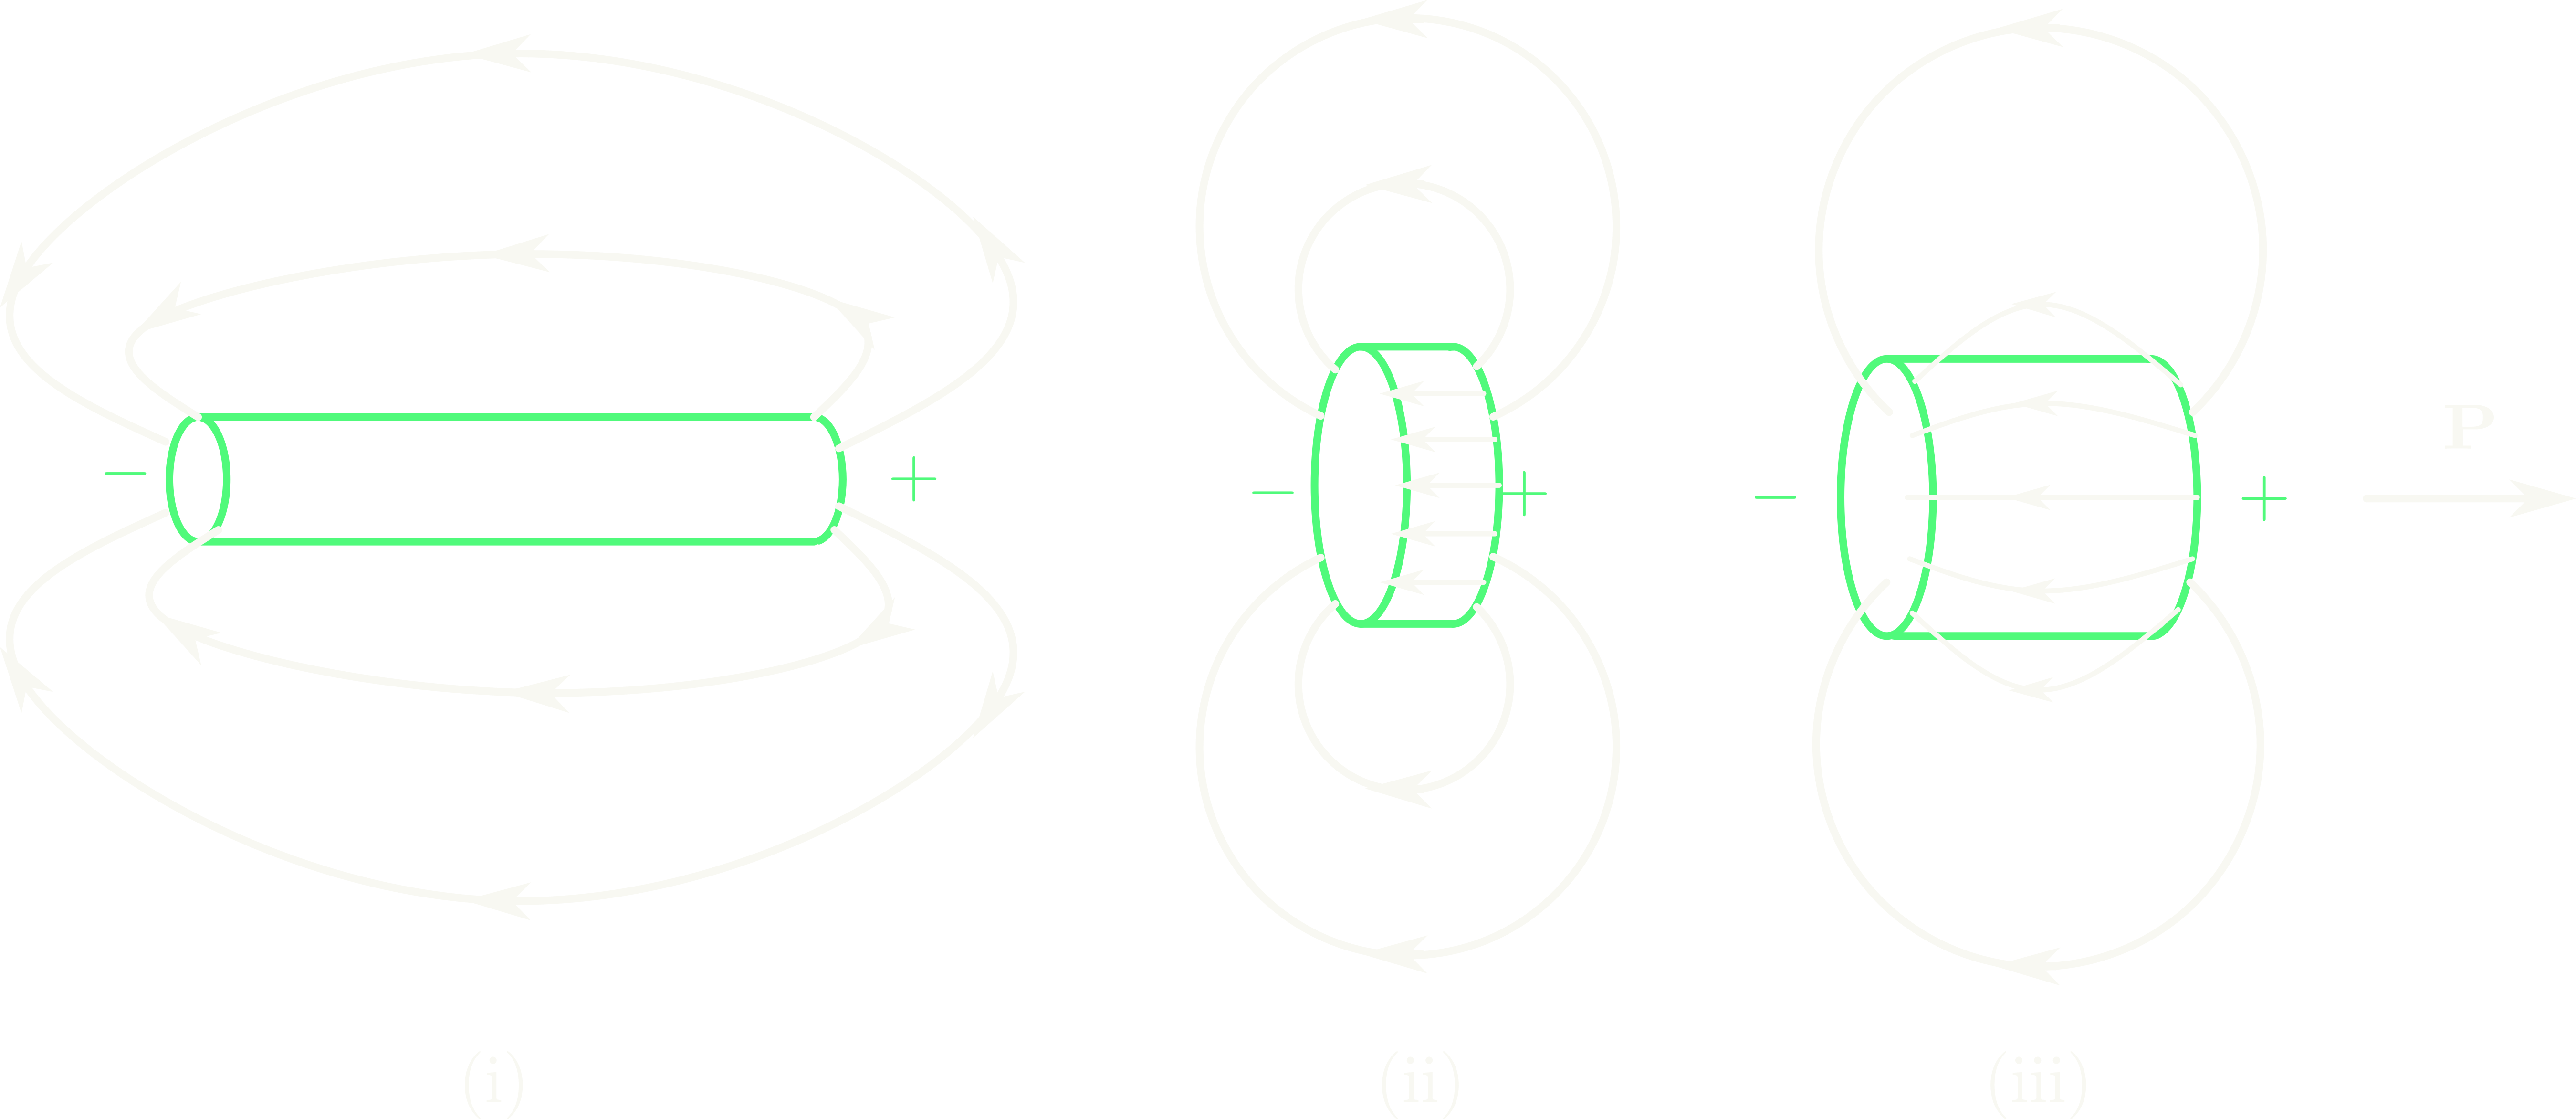
\includegraphics[width=0.8\linewidth]{hw4_11.png}
        \captionsetup{width=0.8\linewidth}
        \caption{Sketch of E-field for a short cylinder}
    \end{figure*}
\end{itemize}

\newpage
\paragraph{4.14} Given
\begin{align*} \tag{4.11, 4.12} \label{eq:11_12}
    \sigma_b \equiv \vb P \cdot \vu n, \quad \rho_b \equiv -\div \vb P
\end{align*}
Polarizing a neutral dielectric moves the charge a bit, so total bound charge is
\begin{align*}
    Q &= \oint_S \sigma_b \dd{\vb a} + \int_V \rho_b \dd{\tau} \\
    &= \oint_S \vb P \cdot \dd{a} - \int_V \div \vb P \dd{\tau} = 0
\end{align*}
from the divergence theorem $\int \div \vb P \dd{\tau} = \oint \vb P \cdot \dd{a}$, so the total bound charge vanishes.

\newpage
\paragraph{4.34} A dielectric cube of side $a$ centered at the origin with a ``frozen-in'' polarization $\vb P = k \vb r$ where $k$ is a constant
and $\vb r = x \vu x + y \vu y + z \vu z$.

First the volume bound charge density is
\begin{align*}
    \rho_b = -\div \vb P = -\div (k \vb r) = -k \qt(\pdv{x} x + \pdv{y} y + \pdv{z} z) = -3k
\end{align*}
and the surface bound charge density is, e.g. on the face $\vu n = \vu x, \quad x = a/2$,
\begin{align*}
    \sigma_b = \vb P \cdot \vu n = \frac{k a}{2}
\end{align*}
which is the same for all six faces. The total bound charge is 
\begin{align*}
    Q = \int_V \rho_b \dd{\tau} + \oint_S \sigma_b \dd{a} = -3k a^3 + \frac{k a}{2} (6a^2) = 0
\end{align*}
where the volume integral is just the volume of the cube $a^3$ and the surface integral is the sum of the areas of the six faces $6a^2$.
\end{document} 